% Slug: four-of-diamonds
% Description: ?
% Author: Cisco
% Story: Cisco
% Test Data: Cisco
% Testers: ?
% Editorial: ?
% TempSlug: four-of-diamonds

% Please don't modify or delete TempSlug

\problem{Absolute Cinema}

For Bob's art class, he was tasked with making art of a mountain range---but, it must be done in a creative way, and the more creative the better.  Alice suggests that he could model the mountain range using mathematics!

Given a sequence $a_1, a_2, a_3, \dots, a_n$ of non-negative \textbf{even} integers, let
\begin{align*}
    A(x) &= \min\left(|x - a_1|,~|x - a_2|,~|x - a_3|, \dots, ~|x - a_n|\right).
\end{align*}
Alice says that this function $A(x)$ resembles a mountain range when its graph is plotted using a graphing calculator!

For example, if $a = [6, 2, 8, 2]$, then the graph of $$
    A(x) = \min(|x-6|,~|x-2|,~|x-8|,~|x-2|)
$$ would be the one illustrated below.
\begin{center}
    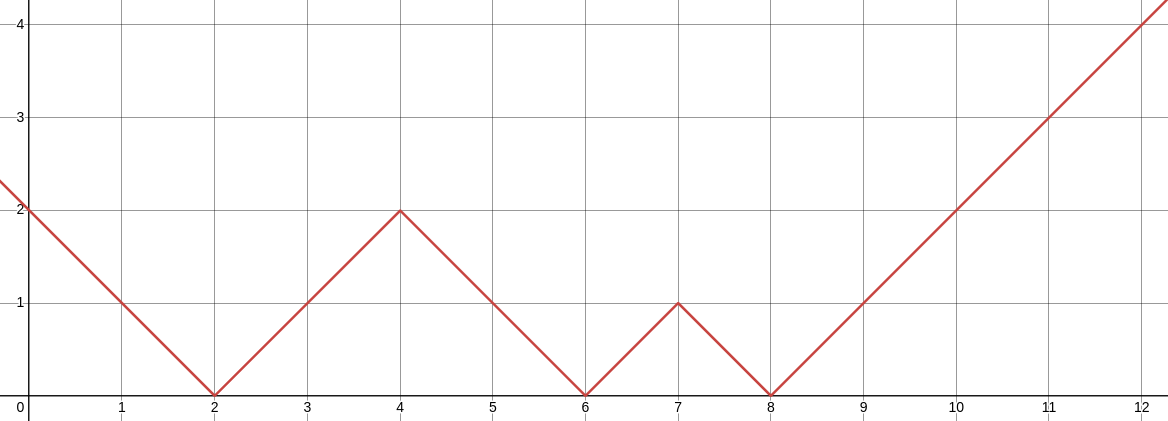
\includegraphics[width=0.75\linewidth]{img/absolute-0e.png}
\end{center}

Bob would like to create a mountain range by defining the function $A(x)$ using his favorite integer sequence $a_1, a_2, a_3, \dots, a_n$.  His painting will span from $x=0$ to $x=r$, and he will use green paint to shade in the region between $A(x)$ and the $x$-axis.

For example, if $a = [3, 1, 4, 1]$ and $r=6$, then the Bob would want to paint green the highlighted region in the diagram below.
\begin{center}
    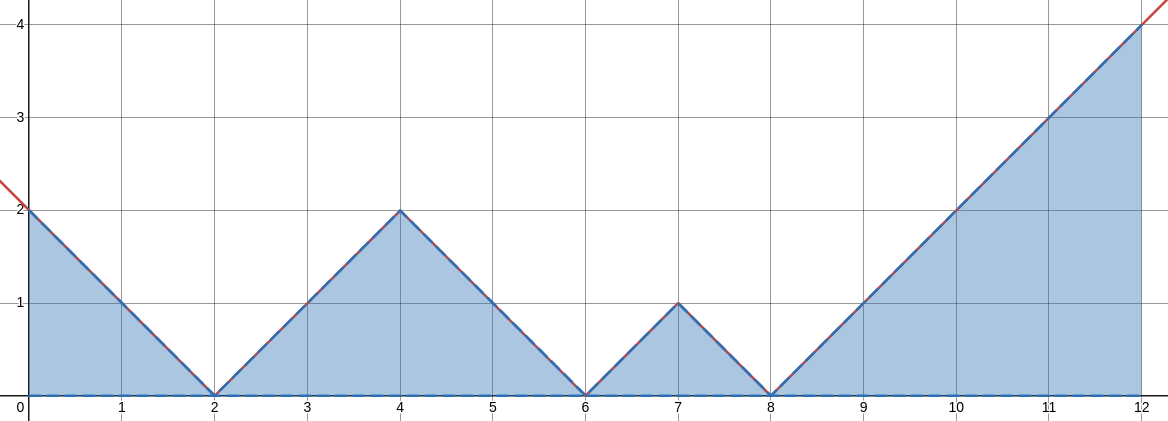
\includegraphics[width=0.75\linewidth]{img/absolute-1e.png}
\end{center}
Its total area can be shown to be \texttt{15} exactly.  In fact, Bob is able to show that if the $a_i$ are all even, then the area of the desired region is \textbf{guaranteed} to be an integer!

Given all these values, please determine the total \textit{area} of this region, so that Bob knows how much paint to buy.  It's \textit{integral} that he knows this information, \textit{definitely}!

\newpage

\subsection*{Input Format}

Input begins with a single line containing the space-separated integers $n$ and $r$.

The second line of input contains the $n$ space-separated integers $a_1, a_2, a_3, \dots, a_n$.

\subsection*{Output Format}

Output a line containing a single real number, the area of the desired region (rounded to exactly two decimal places).

\subsection*{Constraints}

\textit{Your program will only be tested on data that satisfies the following constraints.}

% Set to (10^5, 10^9) in true bounds
\constraints{
    $1 \leq n \leq 100$ \\
    $1 \leq r \leq 1000$ \\
}

\textit{There is no need to validate in your program that these constraints hold.}

\subsection*{Sample I/O}

\begin{sampleIO}
\begin{verbatim}
4 6
3 1 4 1
\end{verbatim}
&
\begin{verbatim}
3.75
\end{verbatim}
\end{sampleIO}

\begin{sampleIO}
\begin{verbatim}
1 2
1
\end{verbatim}
&
\begin{verbatim}
1.00
\end{verbatim}
\end{sampleIO}


% \subsection*{Explanation}
